\documentclass{beamer}

% --- Presentation Theme ---
\usetheme{default} % A clean, professional theme with navigation bars.
%\usecolortheme{beaver} % A pleasant, high-contrast color scheme.
\setbeamercolor{block title}{bg=blue!20!white,fg=black} % Lighter block titles
\setbeamercolor{block body}{bg=blue!5!white}
\setbeamercovered{transparent} % Fades out unrevealed items.

% --- Packages ---
\usepackage[utf8]{inputenc}
\usepackage{amsmath}
\usepackage{amssymb}
\usepackage{amsfonts}
\usepackage{tikz}
\usetikzlibrary{calc, shapes.geometric}
\usepackage{braket}      % For professional quantum mechanics notation (e.g., \ket{}, \bra{})
\usepackage{siunitx}     % For consistent and well-formatted units (e.g., \SI{1.585}{bits})

% --- Custom Commands for Consistency ---
\newcommand{\Hfull}{H_{\text{full}}}
\newcommand{\Hcoll}{H_{\text{coll}}}
\newcommand{\HcaseA}{H_{\text{case A}}}
\newcommand{\HcaseB}{H_{\text{case B}}}
\newcommand{\obs}[1]{#1_{\text{obs}}} % For observed states

% --- Metadata ---
\title{Chromatic ``Operator-Valued'' Contextuality}
\author{Karl Svozil}
\institute{Institute for Theoretical Physics, TU Wien, Vienna}
\date{QIP25, V\"axj\"o, Sweden \textbullet{} 2025-06-10\\ $\;$\\
\url{http://tph.tuwien.ac.at/~svozil/publ/2025-Vaxjoe-pres-Svozil.pdf}}

\begin{document}

% --- Title Page ---
\begin{frame}
    \titlepage
\end{frame}

%==================================================================
\section{Understanding Information}
%==================================================================
\begin{frame}{Shannon Entropy: Quantifying Information}
    \begin{itemize}
        \item Shannon Entropy ($H$) measures the \alert{average uncertainty} or \alert{information content} of a random variable.
        \item The more uncertain an outcome, the higher its entropy, and the more information we gain upon observation.
        \item It's typically measured in \alert{bits} (when using $\log_2$).
    \end{itemize}
    \pause
    \begin{block}{Formula for Shannon Entropy}
        For a discrete random variable $X$ with outcomes $x_i$ and probabilities $P(x_i)$:
        \begin{equation*}
            H(X) = -\sum_{i=1}^{n} P(x_i) \log_2 P(x_i)
        \end{equation*}
    \end{block}
    \pause
    \begin{alertblock}{Core Assumption}
        For the following examples, we assume the initial underlying states are \textbf{equiprobable}.
    \end{alertblock}
\end{frame}

%==================================================================
\section{3-State System Analysis}
%==================================================================
\begin{frame}{3-State System: Full Resolution}
    \begin{itemize}
        \item \textbf{System:} 3 distinct, equiprobable states.
        \item \textbf{Observed Outcomes:} $\{0, 1, 2\}$
        \item \textbf{Probabilities:} $P(0) = P(1) = P(2) = 1/3$
    \end{itemize}
    \pause
    \begin{block}{Calculating Information ($\Hfull$)}
        \begin{align*}
            \Hfull &= - \sum_{i=0}^{2} \frac{1}{3} \log_2 \left(\frac{1}{3}\right) \\
            &= -3 \times \frac{1}{3} \log_2 \left(\frac{1}{3}\right) = \log_2(3) \\
            &\approx \SI{1.585}{bits}
        \end{align*}
    \end{block}
\end{frame}

\begin{frame}{3-State System: Aggregated Resolution}
    \begin{itemize}
        \item \textbf{Mapping (Aggregation):}
             $0 \to \obs{0}$, \quad $1 \to \obs{1}$, \quad $2 \to \obs{1}$
        \item \textbf{New Observed Outcomes:} $\{\obs{0}, \obs{1}\}$
        \item \textbf{New Probabilities:}
            \begin{align*}
                P(\obs{0}) &= P(0) = 1/3 \\
                P(\obs{1}) &= P(1) + P(2) = 2/3
            \end{align*}
    \end{itemize}
    \pause
    \begin{block}{Calculating Information ($\Hcoll$)}
        \begin{align*}
            \Hcoll &= - \left[ \frac{1}{3} \log_2 \left(\frac{1}{3}\right) + \frac{2}{3} \log_2 \left(\frac{2}{3}\right) \right] \\
            &\approx \SI{0.918}{bits}
        \end{align*}
    \end{block}
\end{frame}

\begin{frame}{3-State System: Summary}
    \begin{columns}[T] % Aligns the top of the columns
        \begin{column}{0.5\textwidth}
            \begin{itemize}
                \item \textbf{Full Resolution:} \\ $\Hfull \approx \alert{\SI{1.585}{bits}}$
                \vspace{1em}
                \item \textbf{Aggregated Resolution:} \\ $\Hcoll \approx \alert{\SI{0.918}{bits}}$
            \end{itemize}
        \end{column}
        \begin{column}{0.5\textwidth}
            \pause
            \begin{block}{Information Loss}
                The aggregation reduces the information obtained.
                \begin{align*}
                    \text{Loss} &= \Hfull - \Hcoll \\
                    &\approx 1.585 - 0.918 \\
                    &= \mathbf{\SI{0.667}{bits}}
                \end{align*}
            \end{block}
        \end{column}
    \end{columns}
\end{frame}

%==================================================================
\section{4-State System Analysis}
%==================================================================
\begin{frame}{4-State System: Full Resolution}
    \begin{itemize}
        \item \textbf{System:} 4 distinct, equiprobable states.
        \item \textbf{Observed Outcomes:} $\{0, 1, 2, 3\}$
        \item \textbf{Probabilities:} $P(0) = P(1) = P(2) = P(3) = 1/4$
    \end{itemize}
    \pause
    \begin{block}{Calculating Information ($\Hfull$)}
        \begin{align*}
            \Hfull &= - \sum_{i=0}^{3} \frac{1}{4} \log_2 \left(\frac{1}{4}\right) = \log_2(4) \\
            &= \SI{2}{bits}
        \end{align*}
        \alert{A 4-state equiprobable system perfectly encodes 2 bits.}
    \end{block}
\end{frame}

\begin{frame}{4-State System: Aggregated Cases}
    \begin{columns}[T]
        \begin{column}{0.5\textwidth}
            \begin{block}{Case A: Symmetric Aggregation}
                $\{0, 1\} \to \obs{0}$ \\
                $\{2, 3\} \to \obs{1}$
                \pause
                \begin{align*}
                    P(\obs{0}) &= 1/2 \\
                    P(\obs{1}) &= 1/2 \\
                    \HcaseA &= \SI{1}{bit}
                \end{align*}
                \alert<3>{Like a fair coin flip.}
            \end{block}
        \end{column}
        \begin{column}{0.5\textwidth}
            \pause
            \begin{block}{Case B: Asymmetric Aggregation}
                $\{0, 1, 2\} \to \obs{0}$ \\
                $\{3\} \to \obs{1}$
                \pause
                \begin{align*}
                    P(\obs{0}) &= 3/4 \\
                    P(\obs{1}) &= 1/4 \\
                    \HcaseB &\approx \SI{0.811}{bits}
                \end{align*}
            \end{block}
        \end{column}
    \end{columns}
\end{frame}


\begin{frame}{4-State System: Summary}
    \begin{itemize}
        \item \textbf{Full Resolution:} $\Hfull = \alert{\SI{2}{bits}}$
        \item \textbf{Case A (Symmetric):} $\HcaseA = \alert{\SI{1}{bit}}$
        \item \textbf{Case B (Asymmetric):} $\HcaseB \approx \alert{\SI{0.811}{bits}}$
    \end{itemize}
    \pause
    \begin{block}{Observation}
        Each state aggregation leads to a \alert{reduction} in measurable information. The more states are merged and the more skewed the resulting probabilities, the lower the entropy.
    \end{block}
\end{frame}

%==================================================================
\section{Quantum Contextuality}
%==================================================================
\begin{frame}{2-Valued States in 3 Dimensions}
    \begin{columns}[c] % Vertically center columns
        \begin{column}{0.45\textwidth}
            \resizebox{\textwidth}{!}{
                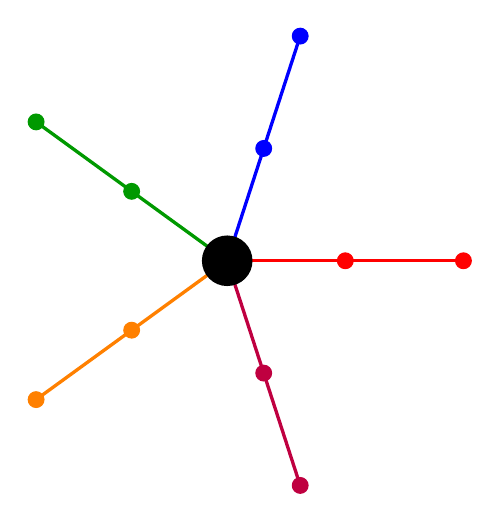
\begin{tikzpicture}
                  % --- Definitions ---
                  \def\centralRadius{0.3cm}
                  \def\rayLength{3cm}
                  \def\smallCircleRadius{0.1cm}
                  \def\lineWidth{very thick}

                  % --- Rays and Outer Circles ---
                  % CORRECTED 'Green' to 'green' (lowercase) to avoid package error.
                  \foreach \angle/\rayColor in {0/red, 72/blue, 144/green!60!black, 216/orange, 288/purple} {
                    \draw[color=\rayColor, \lineWidth] (0,0) -- (\angle:\rayLength);
                    \filldraw[color=\rayColor] (\angle:{\rayLength/2}) circle (\smallCircleRadius);
                    \filldraw[color=\rayColor] (\angle:\rayLength) circle (\smallCircleRadius);
                  }
                  % --- Central Atom ---
                  \filldraw[black, \lineWidth] (0,0) circle (\centralRadius);
                \end{tikzpicture}
            }
        \end{column}
        \begin{column}{0.55\textwidth}
            \begin{block}{Interpretation}
            This represents a aggregated system:
            \begin{itemize}
                \item The \alert{black} state maps to value 1.
                \item All \alert{non-black} states map to value 0.
            \end{itemize}
            In Hilbert space, this corresponds to projecting onto a 1D subspace vs. its orthogonal (d-1)D complement.
            \end{block}
        \end{column}
    \end{columns}
\end{frame}

\begin{frame}{Spectral Decomposition: Maximal vs. Degenerate, ``full operator-valued versus two-valued'' }
    Let $\{\ket{\mathbf{e}_i} \mid 1 \le i \le d\}$ be an orthonormal basis.
    \begin{block}{Maximal Operator (von Neumann, 1931)}
    Outcomes $\lambda_i$ are mutually distinct (unique "colors"):
    \[ A = \sum_{i=1}^d \lambda_i \ket{\mathbf{e}_i}\bra{\mathbf{e}_i} \]
    \end{block}
    \pause
    \begin{block}{Degenerate Operator (Projector)}
    Only two outcomes (e.g., 1 for state $j$, 0 otherwise):
    \[ P_j = \ket{\mathbf{e}_j}\bra{\mathbf{e}_j} = \sum_{i=1}^d \delta_{ij} \ket{\mathbf{e}_i}\bra{\mathbf{e}_i} \]
    \end{block}
\end{frame}

\begin{frame}{Postulate/Presumption of Classicality}
\begin{itemize}
        \item \textbf{Chromatic Noncontextuality:} The color (value) of intertwining observables is independent of the (hyper)edge.
        \item \textbf{Chromatic Reality:} Existence of classical $d$-ary elements of physical reality for certain $d$-uniform
"chromatic Kochen-Specker" hypergraphs.
    \end{itemize}
\end{frame}

\begin{frame}{Results on Chromatic Contextuality}
    \begin{itemize}[<+->] % Reveals items one by one
        \item If a ($d$-uniform hyper)graph has chromatic number $d$, it has at least $d$ two-valued states (by aggregation). \\ \footnotesize (M. H. Shekarriz and KS, JMP 63, 032104, 2022)
        \item The Yu-Oh 3-uniform (hyper)graph has clique number 3 but chromatic number 4, yet is set representable. This is a "Chromatic Kochen-Specker theorem". \\ \footnotesize (KS, Entropy 27, 387, 2025)
        \item The house/pentagon/pentagram $d$-uniform hypergraph has one "exotic" 2-valued state that cannot be obtained by aggregating one of its 5 non-equivalent colorings. \\ \footnotesize (KS, Entropy 27, 387, 2025)
    \end{itemize}
\end{frame}

%==================================================================
\section{Summary}
%==================================================================
\begin{frame}{Summary}
    \begin{beamercolorbox}[sep=2em,center]{block body}
        \huge\alert{Colorings are a formidable tool to investigate quantum contextuality.}
    \end{beamercolorbox}
\end{frame}

\end{document}
